\documentclass[tikz]{standalone}
\usepackage{pgfplots}
\pgfplotsset{compat=1.15}
\usepackage{mathrsfs}
\usetikzlibrary{arrows,calc}
\usepackage{tkz-euclide}
\pagestyle{empty}

\definecolor{AngleClr}{rgb}{0,0.39215686274509803,0}
\definecolor{ShapeClr}{rgb}{0.6,0.2,0}
\definecolor{BlueSqr}{RGB}{5,81,163}
\definecolor{RedSqr}{RGB}{0, 156, 0}

\newcommand{\add}[2]{\dimexpr#1+#2\relax}

\begin{document}

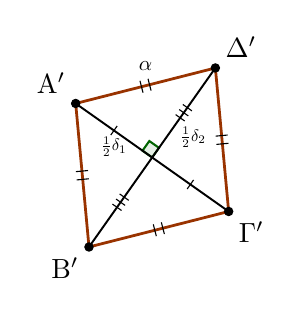
\begin{tikzpicture}[scale=.75]
\tkzSetUpLine[line width=1pt,color=black]
\tkzSetUpPoint[fill=black]

\tkzDefPoints{0/0/B,3.5/0/C,0.95/1.8/A,2.75/2.25/D}

\tkzCalcLength(A,B)\tkzGetLength{dAB}
\tkzCalcLength(C,B)\tkzGetLength{dCB}

\tkzCalcLength(A,D)\tkzGetLength{dAD}
\tkzCalcLength(C,D)\tkzGetLength{dCD}

\pgfmathsetmacro{\dOne}{(\dAB+\dCB)/2}
\pgfmathsetmacro{\dTwo}{(\dAD+\dCD)/2}

\pgfmathsetmacro{\dThree}{(\dOne + \dTwo)/2}

% \tkzInterCC[R](A,(\dAB + \dCB)/2)(C,(\dAB + \dCB)/2) \tkzGetPoints{X}{Y}
\tkzInterCC[R](A,\dOne)(C,\dOne) \tkzGetPoints{X}{B'}
\tkzInterCC[R](A,\dTwo)(C,\dTwo) \tkzGetPoints{D'}{Y}

\tkzInterCC[R](B',\dThree)(D',\dThree) \tkzGetPoints{A'}{C'}

\tkzInterLL(A',C')(B',D') \tkzGetPoint{I}

\tkzFillPolygon[fill=white](A',B',C',D')
\tkzMarkRightAngle[line width=0.75pt, size=.2,color=AngleClr,fill=AngleClr,fill opacity=0.1](A',I,D')
\tkzDrawSegments[line width=0.7pt](A',C' B',D')

% \tkzDrawPolygon[color=ShapeClr,line width=0.5pt](A,B',C,D')
\tkzDrawPolygon[color=ShapeClr](A',B',C',D')
\tkzDrawPoints[size=3](B',D',A',C')
\tkzLabelPoint[above left](A'){$\rm A'$}
\tkzLabelPoint[below left](B'){$\rm B'$}
\tkzLabelPoint[below right](C'){$\rm \Gamma'$}
\tkzLabelPoint[above right](D'){$\rm \Delta'$}

\tkzMarkSegments[mark=||,size=2.2](A',D' C',D' A',B' C',B')
\tkzMarkSegments[mark=|,size=2](I,A' I,C')
\tkzMarkSegments[mark=|||,size=2](I,B' I,D')

\tkzLabelSegment[yshift=0.4cm,scale=0.75](A',D'){$\alpha$}
\tkzLabelSegment[scale=0.6](A',I){$\frac{1}{2}\delta_1$}
\tkzLabelSegment[scale=0.6,yshift=-0.18cm,xshift=0.2cm](D',I){$\frac{1}{2}\delta_2$}

\end{tikzpicture}

\end{document}
